%
% Introduction
%

\section{Introduction} \label{sec:introduction}

The internet is one of the key technological achievements of the 20th century, an enabling factor in every aspect of our everyday use of modern technology. While digital computing was the definitive technology of the 20th century, quantum technologies will be for the 21st \cite{bib:NielsenChuang00, bib:Bennett00}. 

Perhaps the most exciting prospect in the quantum age is the development of quantum computers\index{Quantum computing}. Richard Feynman \cite{bib:Feynman85} was the first to ask the question `If quantum systems are so exponentially complex that we are unable to simulate them on our classical computers, can those same quantum systems be exploited in a controlled way to exponentially outperform our classical computers?'\index{Richard Feynman}. Subsequently, the Deutsch-Jozsa algorithm \cite{bib:DeutschJozsa92}\index{Deutsch-Jozsa algorithm} demonstrated for the first time that algorithms can run on a quantum computer, exponentially outperforming any classical algorithm. Since then, an enormous amount of research has been dedicated to finding new quantum algorithms, and the search has indeed been a very fruitful one\footnote{See the Quantum Algorithm Zoo\index{Quantum Algorithm Zoo} for a comprehensive summary of the current state of knowledge on quantum algorithms (\texttt{\href{http://math.nist.gov/quantum/zoo/}{http://math.nist.gov/quantum/zoo/}}).}, with many important applications having been found, including, amongst many others\index{Quantum algorithms}:

\begin{itemize}
	\item Searching unstructured databases (Sec.~\ref{sec:quantum_search}):\index{Grover's algorithm}
		\begin{itemize}
		\item Grover's algorithm \cite{bib:Grover96}.
		\item Quadratic speedup.
		\end{itemize}
	\item Satisfiability \& optimisation problems\footnote{A satisfiability problem is one where we search a function's input space for a solution(s) satisfying a given output constraint. The hardest such problems, like the archetypal 3-\textsc{SAT}\index{3-SAT problem} problem, are \textbf{NP}-complete.}\index{\textbf{NP} \& \textbf{NP}-complete} (Sec.~\ref{sec:optimising_the_world}):
		\begin{itemize}
			\item Grover's algorithm.
			\item Quadratic speedup.
			\item Includes solving \textbf{NP}-complete problems, and brute-force cracking of private encryption keys.\index{Satisfiability problems}
			\item Many optimisation problems are \textbf{NP}-complete or can be approximated in \textbf{NP}-complete.\index{Optimisation problems}
			\end{itemize}
	\item Period finding and integer factorisation\index{Shor's algorithm} (Sec.~\ref{sec:shors_alg}):
		\begin{itemize}
		\item Shor's algorithm \cite{bib:ShorFactor}.
		\item Exponential speedup.
		\item This compromises Rivest, Shamir \& Adleman (RSA) public-key cryptography \cite{bib:RSA}\index{RSA encryption}\index{Public-key encryption}, the most widely used cryptographic protocol on the internet today.
		\end{itemize}
	\item Simulation of quantum systems\index{Quantum simulation} (Sec.~\ref{sec:quantum_sim_alg}):
		\begin{itemize}
			\item Lloyd's algorithm \cite{bib:lloyd1996universal}.
			\item Exponential speedup.
			\item This includes simulation of: molecular and atomic interactions in the study of quantum chemistry or nuclear physics; interactions between drug molecules and organic molecules for drug design; genetic interactions for the study of genetics and genetic medicine; nanoscale semiconductor physics for integrated circuit design; and much more.
			\end{itemize}
	\item Simulation of quantum field theories\index{Simulating quantum field theories}:
		\begin{itemize}
		 \item Jordan-Lee-Preskill algorithm \cite{bib:JLP, bib:RohdeWavelet15}
		 \item Exponential speedup.
		 \item A key area of fundamental physics research.
		 \end{itemize}
	\item Topological big-data analysis (Sec.~\ref{sec:TDA}):\index{Topological big-data analysis}
		\begin{itemize}
		\item Lloyd's algorthm \cite{bib:lloyd2016quantum, USTCexperiment}.
		\item Exponential speedup.
		\item Broad applications including: social media network analysis; consumer behaviour; behavioural dynamics; neuroscience; and higher-dimensional signal and image processing.
		\end{itemize}
	\item Solving linear systems of equations (Sec.~\ref{sec:linear_systems}):\index{Linear systems}
		\begin{itemize}
		\item \comment{To do} \cite{bib:harrow2009quantum, bib:BerryLinear}.
		\item Exponential speedup.
		\item Widespread applications in linear algebra and calculus.
		\end{itemize}
	\item Quantum machine learning (Sec.~\ref{sec:quantum_mind}):\index{Quantum machine learning}
		\begin{itemize}
		\item Lloyd's algorithm \cite{bib:lloyd2013quantum}.
		\item This includes putting an end to humanity.
		\item \textit{Ne obliviscaris}.\index{Latin}
		\end{itemize}
\end{itemize}
An elementary technical overview of some of these archetypal algorithms is presented in Sec.~\ref{sec:quantum_algs}.

It is likely we haven't yet begun to fully recognise the capabilities of quantum computers, and the full plethora of applications they may have in the future. We stand at the beginning of the emergence of an entirely new type of technology.

In addition to many practical applications, the onset of quantum computing carries with it deep philosophical implications. Specifically, the Extended Church-Turing (ECT)\index{Extended Church-Turing (ECT) thesis} thesis hypothesises that any physically realisable system can be \textit{efficiently}\footnote{The term `efficient' is one coined by the computer scientist to mean that a problem can be solved in time at most polynomial in the size of the problem.\index{Computational efficiency}} simulated by a universal Turing machine\index{Turing machines} (i.e classical computer). The believed exponential complexity of quantum systems inclines quantum computer scientists to believe that the ECT thesis is therefore false \cite{bib:Deutsch85}\footnote{We have discovered a truly marvellous proof of this, which this footnote is too narrow to contain.}. The demonstration of large-scale quantum computers, while unable to prove or disprove the ECT thesis\footnote{When one talks about `scalability' or the `ECT thesis', we are talking about asymptotic relationships. Clearly no finite-sized experiment can prove asymptotic scaling with certainty. But with a sufficiently large quantum computer at our disposal, demonstrating exponentially more computational power than its classical sibling, we might be reasonably satisfied in convincing ourselves about the nature of the scaling of different computational models.}, could at least provide some convincing evidence against the ECT conjecture.

From a computational complexity\index{Computational complexity theory} theorist's perspective, it is strongly believed that the complexity classes of problems efficiently solvable on classical computers (\textbf{P} \& \textbf{BPP}\index{\textbf{P} \& \textbf{BPP}}) and quantum computers (\textbf{BQP}\index{\textbf{BQP} \& \textbf{BQP}-complete}) are distinct. Specifically, it is believed that \mbox{$\mathbf{BPP}\subset\mathbf{BQP}$}. If this conjecture is correct, it implies the existence of quantum algorithms super-polynomially faster than the best classical ones, and that the ECT thesis is not correct. More specifically, Fig.~\ref{fig:complexity_classes} illustrates the believed relationships between some of the most important complexity classes relevant to quantum computing.

\begin{figure}[!htb]
	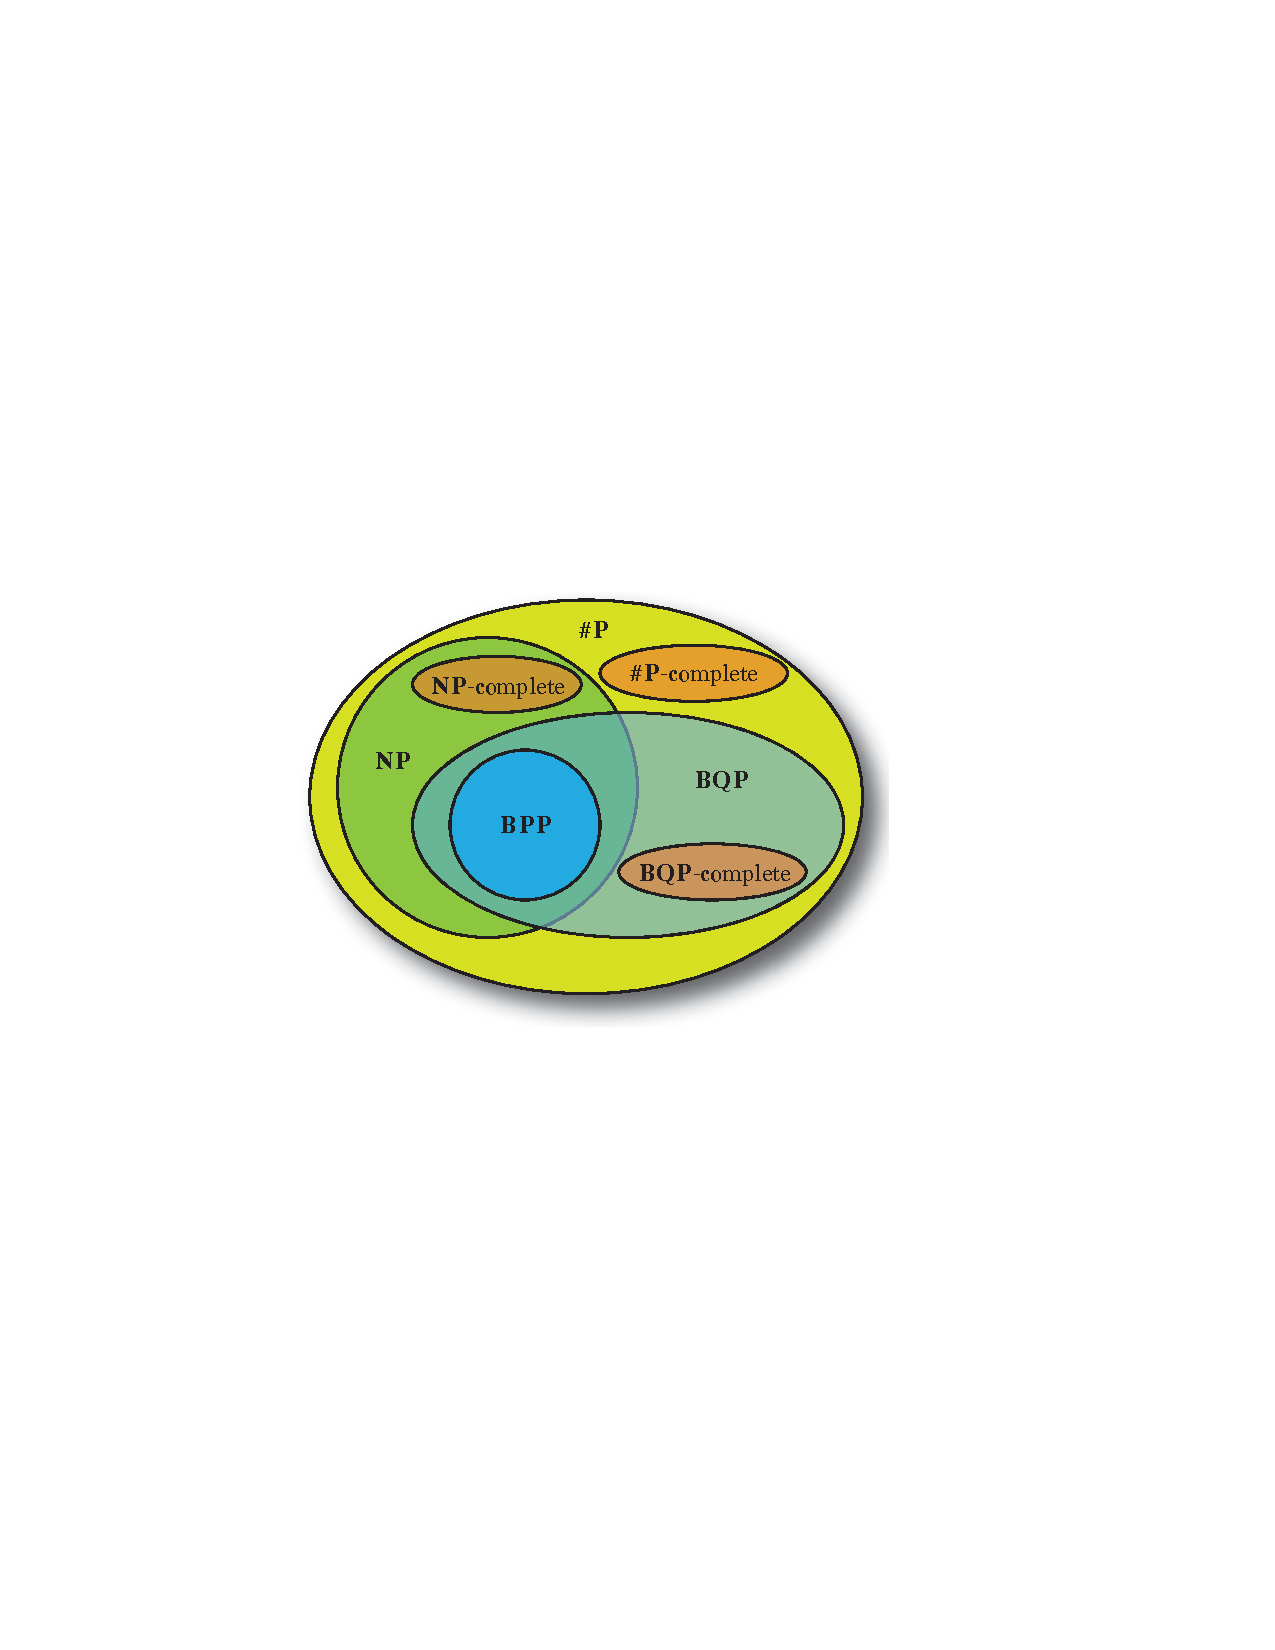
\includegraphics[width=0.5\textwidth]{complexity_classes}\index{Complexity classes} \index{\textbf{P} \& \textbf{BPP}} \index{\textbf{NP} \& \textbf{NP}-complete} \index{\textbf{BQP} \& \textbf{BQP}-complete} \index{\textbf{\#P} \& \textbf{\#P}-complete}
	\caption{Believed relationships between the complexity classes most relevant to quantum computing. \textbf{BPP} is the class of polynomial-time probabilistic classical algorithms. \textbf{NP} is the class of problems verifiable in polynomial time using classical algorithms. \textbf{NP}-complete are the subset of \textbf{NP} problems polynomial-time reducible to any other problem in \textbf{NP}. \textbf{BQP} is the class of probabilistic algorithms solvable in polynomial time on universal quantum computers. $\#\mathbf{P}$ is the set of counting problems, that count satisfying solutions to \textbf{P} problems (\textbf{P} is the same as \textbf{BPP}, but deterministic, rather than probabilisitic). Note that it is actually unproven whether \mbox{$\mathbf{P}=\mathbf{BPP}$} or \mbox{$\mathbf{P}\subset\mathbf{BPP}$}. There are examples where the best known \textbf{BPP} algorithms outperform the best known \textbf{P} algorithms, which could arise because the two classes are inequivalent, or that we simply haven't tried hard enough to find the best deterministic algorithms. Furthermore, while it is known that \mbox{$\mathbf{P}\subseteq\mathbf{NP}$}, it is not known whether \mbox{$\mathbf{BPP}\subseteq\mathbf{NP}$}. For the sake of illustration in our Venn diagram we have taken the view that it is. \textbf{BPP} is regarded as the class of problems efficiently solvable on universal Turing machines (i.e classical computers), whereas \textbf{BQP} is that efficiently solvable on universal quantum computers. The computational superiority of quantum computers is based on the (strongly believed, yet unproven) assumption that \mbox{$\mathbf{BPP}\subset\mathbf{BQP}$}.} \label{fig:complexity_classes}
\end{figure}

Aside from quantum computing, quantum cryptography\index{Quantum cryptography} holds the promise of uncrackable cryptographic protocols, guaranteed not by the assumed complexity of solving certain mathematical problems like integer factorisation or brute-force searching, but by the laws of quantum mechanics. That is, provided our understanding of quantum mechanics is correct, quantum cryptographic protocols exist, which cannot be cracked, irrespective of the computational resources of an adversary.

Already we are beginning to see elementary realisations of essential quantum technologies such as quantum computing, cryptography, and metrology. As these technologies become increasingly viable and more ubiquitous, the demand for networking them and sharing quantum resources between them will become a pressing issue. Most notably, quantum cryptography and \textit{cloud quantum computing} will be pivotal in the proliferation of quantum technology, which necessarily requires reliable quantum communications channels.

The first demonstrations of digital computer networks were nothing more than simple two-party, point-to-point (P2P) communication. However, the internet we have today extends far beyond this, allowing essentially arbitrary worldwide networking across completely ad hoc networks comprising many different mediums, with any number of parties, in an entirely plug-and-play and decentralised fashion. Similarly, elementary demonstrations of quantum communication\index{Quantum communication} have been performed across a small number of parties, and much work has been done on analysing quantum channel capacities in this context \cite{??? channel_capacity}. But, as with digital computing, demand for a future \textit{quantum internet} is foreseeable, enabling the arbitrary communication of quantum resources, between any number of parties, over ad hoc networks.

The digital internet may be considered a technology stack, such as TCP/IP (Transmission Control Protocol/Internet Protocol)\index{Transmission Control Protocol/Internet Protocol (TCP/IP)}, comprising different levels of abstraction of digital information \cite{bib:TanenbaumNet}. At the lowest level we have raw digital data we wish to communicate across a physical medium. Above this, we decompose the data into packets. The packets are transmitted over a network, and TCP is responsible for routing the packets to their destination, and guaranteeing data integrity and Quality of Service (\textsc{QoS}). Finally, the packets received by the recipient are combined and the raw data reconstructed.

The TCP layer remains largely transparent to the end-user, enabling virtual software interfaces to remote digital assets that behave as though they were local. This allows high-level services such as the File Transfer Protocol (FTP), the worldwide web, video and audio streaming, and outsourced computation on supercomputers, as though everything was taking place locally, with the end-user oblivious to the underlying networking protocols, which have been abstracted away. To the user, YouTube videos or Spotify tracks behave as though they were held as local copies. And FTP or DropBox allow storage on a distant data centre to be mounted as though it were a local volume. We foresee a demand for these same criteria in the quantum era.

In the context of a quantum internet, packets of data will instead be quantum states, and the transmission control protocol is responsible for guiding them to their destination and ensuring quality control.

Here we present a treatment for such Quantum Transmission Control Protocols (QTCPs)\index{Quantum Transmission Control Protocol (QTCP)} as a theoretical foundation for a future quantum internet. We consider how such ad hoc networks may be described mathematically, how to quantify network performance, and present a QTCP stack for operating it. While the goals of QTCP are similar as for classical TCP, there are major conceptual differences between the classical and quantum internets, owing to the unique properties of quantum states with no classical analogue.

Our treatment of quantum networks will be optics-heavy, based on the reasonable assumption that communications channels will almost certainly be optical, albeit with many possible choices of optical states and mediums. However, this does not preclude non-optical systems from representing quantum information that is not in transit, and we consider such `hybrid' architectures in detail, as well as the interfacing between optical and non-optical systems. Indeed, it is almost certain that future large-scale quantum computers will not be all-optical, necessitating interfacing different physical architectures. We accommodate for this requirement in the design of the QTCP.

Shared quantum entanglement\index{Quantum entanglement} is a primitive resource with direct applications in countless protocols. This warrants special treatment of quantum networks, which do not implement a full QTCP network stack, but instead specialise in just this one task -- entanglement distribution. We will see that such a specialised network will already be immensely useful for a broad range of applications, and its simplicity brings with it many inherent advantages.

The quantum internet will enable advances in the large-scale deployment of quantum technologies. Most notably, in the context of quantum computing it will allow initially very expensive technology to be economically viable and broadly accessible via the outsourcing of computations from consumers who can't afford quantum computers, to well-resourced hosts who can -- \textit{cloud quantum computing}\index{Cloud quantum computing}.

With the addition of recent advances in homomorphic encryption and blind quantum computing\index{Encrypted quantum computation}, such cloud quantum computing can be performed securely, guaranteeing privacy of both data and algorithms, secure even against the host performing the computation. This opens up entirely new economic models and applications for the licensing of compute time on future quantum computers in the cloud.

The unique behaviour of quantum computing, in terms of the super-classical scaling in its computational power, brings with it many important economic and strategic considerations that are extremely important to give attention to in the post-classical world.

But quantum technologies extend far beyond computation. Many other exciting applications for controlled quantum systems exist, with new ones frequently emerging. Thus, the quantum internet will find utility beyond cloud quantum computing, enabling the global exchange of quantum resources and assets. This could include the networking of elementary quantum resources such as state preparation, entanglement sharing, teleportation and quantum measurements, or scale all the way up to massively distributed quantum computation or a global quantum cryptography network.\index{Quantum assets}

It is hard to foresee the future trajectory of quantum technology, much as no one foresaw the advances digital technology has made over the last half century. But it is certain that as the internet transformed digital technology, the quantum internet will define the future of quantum technologies.